\documentclass{article}
\usepackage{amsfonts}
\usepackage{amsmath}
\usepackage{amsthm}
\usepackage{hyperref}
\usepackage{graphicx}
\usepackage{cleveref}
\usepackage{txfonts}

\begin{document}
\section{Neural Networks and Deep Learning}
See \url{https://www.deeplearning.ai/} for the course.
\subsection{Introduction}
Machine learning has different applications
\begin{itemize}
\item real estate, online advertising (standard neural networks)
\item image classification (CNN)
\item audio to text, language translation (RNN)
\item position of other cars in autonomous driving (hybrid)
\end{itemize}

Supervised learning uses data consisting of input (x) and desired output (y).
In supervised learning there is structured data (house price and features)
and unstructured data (images, audio, text).

Traditional approaches hit a performance plateau as more and more data becomes available.
Deep learning is facilitated by
\begin{itemize}
\item larger datasets
\item more computational power
\item algorithmic improvements
\end{itemize}

Geoffrey Hinton's advice:
\begin{itemize}
\item read enough so that you start developing intuitions
\item trust your intuitions
\item never stop programming
\end{itemize}

\subsection{Basics of Neural Network programming}
\subsubsection{Binary Classification}
Logistic regression is an algorithm for binary classification (e.g. y=1 (cat) vs y=0 (no cat)).
The training set consists of samples $(x,y)$ with $x\in\mathbb{R}^{n_x}$ and $y\in\{0,1\}$.
The training set is $(x^{(1)},y^{(1)}), (x^{(2)},y^{(2)}), \ldots, (x^{(m)},y^{(m)})$ with $m=m_{train}$ (or $m=m_{test}$ for the test set).
The training data is represented by the matrix
\begin{equation}
  X=\begin{pmatrix}x^{(1)} & x^{(2)} & \cdots & x^{(m)}\end{pmatrix}\in\mathbb{R}^{n_x\times m}
\end{equation}
The labels are
\begin{equation}
  Y=\begin{pmatrix}y^{(1)} & y^{(2)} & \cdots & y^{(m)}\end{pmatrix}\in\mathbb{R}^{1\times m}
\end{equation}

Logistic regression tries to model the probability $\widehat{y}=P(y=1|x)$.
The model has the parameters $w\in\mathbb{R}^{n_x}$ and $b\in\mathbb{R}$.
The model is $\widehat{y}^{(i)}=\sigma(w^\top x^{(i)}+b)$ using $\sigma(z^{(i)})=\frac{1}{1+e^{-z^{(i)}}}$.
Also see \cref{fig:sigmoid}.
\begin{figure}[htbp]
  \begin{center}
    \includegraphics[width=.5\textwidth]{sigmoid}
    \caption{The sigmoid activation function}
    \label{fig:sigmoid}
  \end{center}
\end{figure}

\subsubsection{Cost function}
The logistic regression \emph{loss function} computes the error for a single training example.
\begin{equation}
  \mathcal{L}(\widehat{y},y)=-\big(y\log\widehat{y}+(1-y)\log(1-\widehat{y})\big)
\end{equation}
with $y\in\{0,1\}$.
The \emph{cost function} is the average of the loss function of the entire training set.
\begin{equation}
  J(w,b)=\frac{1}{m}\sum_{i=1}^m\mathcal{L}(\widehat{y}^{(i)},y^{(i)})=
  -\frac{1}{m}\sum_{i=1}^m\big[y^{(i)}\log\widehat{y}^{(i)}+(1-y^{(i)})\log(1-\widehat{y}^{(i)})\big]
\end{equation}

\subsubsection{Gradient descent}
Gradient descent iteratively minimizes $J(w,b)$ using partial derivatives of $J$.
\begin{equation}
  \begin{split}
    w&\coloneqq w-\alpha\underbrace{\frac{\partial J(w,b)}{\partial w}}_{\eqqcolon dw}\\
    b&\coloneqq b-\alpha\underbrace{\frac{\partial J(w,b)}{\partial b}}_{\eqqcolon db}
  \end{split}
\end{equation}
$\alpha$ is the learning rate.

Derivative chain-rule: $\frac{df(g(x))}{dx}=\frac{df}{dg}\frac{dg}{dx}$.
In the source code $\frac{dJ}{dv}$ is named ``dv'' where $J$ is the final output variable.

In the case of logistic regression with two features $z=w_1x_1+w_2x_2+b$ and $a=\sigma(z)$.
\begin{equation}
  \begin{split}
    \frac{d\mathcal{L}(a,y)}{da}&=-\frac{y}{a}+\frac{1-y}{1-a}\\
    \frac{da}{dz}&=a(1-a)\\
    ``dz''=\frac{d\mathcal{L}}{dz}&=\frac{d\mathcal{L}}{da}\frac{da}{dz}=a-y
  \end{split}
\end{equation}
$\frac{d\mathcal{L}}{dw_1}=``dw_1''=x_1 dz$, $``dw_2''=x_2dz$, and $``db''=dz$.
The update rule for gradient descent then is
\begin{equation}
  \begin{split}
    w_1&\coloneqq w_1-\alpha dw_1\\
    w_2&\coloneqq w_2-\alpha dw_2\\
    b&\coloneqq b-\alpha db\\
  \end{split}
\end{equation}

\subsubsection{Logistic regression on $m$ examples}
Logistic regression over multiple training examples works by simply summing up the derivatives.
\begin{equation}
  \frac{\partial}{\partial w_1}J(w,b)=\frac{1}{m}\sum_{i=1}^m\underbrace{\frac{\partial}{\partial w_1}\mathcal{L}(a^{(i)},y^{(i)})}_{dw_1^{(i)}}
\end{equation}
See \cref{fig:logistic-regression} for more detail.
\begin{figure}
  \begin{center}
    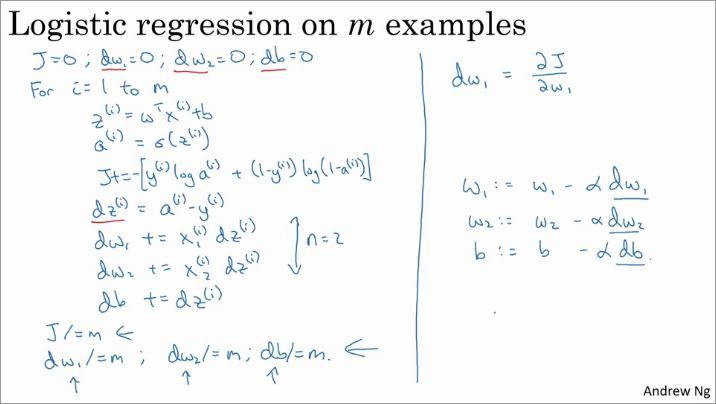
\includegraphics[width=\textwidth]{logistic-regression}
    \caption{Logistic regression on $m$ examples}
    \label{fig:logistic-regression}
  \end{center}
\end{figure}

\subsection{One hidden layer Neural Network}
\subsection{Deep Neural Networks}

\section{Improving Deep Neural Networks: Hyperparameter tuning, Regularisation}
\section{Structuring Machine Learning Projects}
\section{Convolutional Neural Networks}
\section{Sequence Models}

\end{document}
